%%%%%%%%%%%%%%%%%%%%%%%%%%%%%%%%%%%%%%%%%
% Stylish Article
% LaTeX Template
% Version 2.1 (1/10/15)
%
% This template has been downloaded from:
% http://www.LaTeXTemplates.com
%
% Original author:
% Mathias Legrand (legrand.mathias@gmail.com) 
% With extensive modifications by:
% Vel (vel@latextemplates.com)
%
% License:
% CC BY-NC-SA 3.0 (http://creativecommons.org/licenses/by-nc-sa/3.0/)
%
%%%%%%%%%%%%%%%%%%%%%%%%%%%%%%%%%%%%%%%%%

%----------------------------------------------------------------------------------------
%	PACKAGES AND OTHER DOCUMENT CONFIGURATIONS
%----------------------------------------------------------------------------------------

\documentclass[fleqn,10pt]{SelfArx} % Document font size and equations flushed left

\usepackage[english]{babel} % Specify a different language here - english by default

\usepackage{lipsum} % Required to insert dummy text. To be removed otherwise

%----------------------------------------------------------------------------------------
%	COLUMNS
%----------------------------------------------------------------------------------------

\setlength{\columnsep}{0.55cm} % Distance between the two columns of text
\setlength{\fboxrule}{0.75pt} % Width of the border around the abstract

%----------------------------------------------------------------------------------------
%	COLORS
%----------------------------------------------------------------------------------------

\definecolor{color1}{RGB}{0,0,90} % Color of the article title and sections
\definecolor{color2}{RGB}{0,20,20} % Color of the boxes behind the abstract and headings

%----------------------------------------------------------------------------------------
%	HYPERLINKS
%----------------------------------------------------------------------------------------

\usepackage{hyperref} % Required for hyperlinks
\hypersetup{hidelinks,colorlinks,breaklinks=true,urlcolor=color2,citecolor=color1,linkcolor=color1,bookmarksopen=false,pdftitle={Title},pdfauthor={Author}}

%----------------------------------------------------------------------------------------
%	ARTICLE INFORMATION
%----------------------------------------------------------------------------------------

%\JournalInfo{Journal, Vol. XXI, No. 1, 1-5, 2013} % Journal information
%\Archive{Additional note} % Additional notes (e.g. copyright, DOI, review/research article)

\PaperTitle{Commssioning of an automated assembly system for the PS modules of the CMS phase II upgrade outer tracker.} % Article title

\Authors{James Keaveney\textsuperscript{1}*} % Authors
\affiliation{\textsuperscript{1}\textit{DESY, Hamburg Germany}} % Author affiliation
\affiliation{*\textbf{} james.keaveney@desy.de} % Corresponding author

\Keywords{} % Keywords - if you don't want any simply remove all the text between the curly brackets
\newcommand{\keywordname}{Keywords} % Defines the keywords heading name

%----------------------------------------------------------------------------------------
%	ABSTRACT
%----------------------------------------------------------------------------------------

\Abstract{
 The CMS phase II upgrade outer tracker is built from two types of modules (\emph{PS} and \emph{2S}) each consisting of two silicon sensors and associated electronics and mechanics. In the case of the PS module, the sensors be assembled to a precision of approximately 20 microns.  In order to satisfy this requirement and a short module assembly time, an \emph{automated} assembly system is proposed. The student will join an ongoing effort to commission such a system based on a high-precision motion-stage integrated with pattern-recognition and mechanical control systems.  The student will work towards the demonstration of high precision assembly with short assembly times. 
 If time permits, the student will also commission a proposed module metrology system based on the same hardware.

 %extend the system to measure the alignment precision of assembled modules by realising a novel metrology concept that has been established already at the concept level. The student will develop mathematical and a software skills in addition to gaining experience with a state of the art lab environment. The final goal will be to confirm that the  automated assembly procedure achieves the alignment precision demanded by the module design.
}

%----------------------------------------------------------------------------------------

\begin{document}

\flushbottom % Makes all text pages the same height

\maketitle % Print the title and abstract box

\tableofcontents % Print the contents section

\thispagestyle{empty} % Removes page numbering from the first page

%----------------------------------------------------------------------------------------
%	ARTICLE CONTENTS
%----------------------------------------------------------------------------------------

\section*{Introduction} % The \section*{} command stops section numbering




\addcontentsline{toc}{section}{Introduction} % Adds this section to the table of contents
The CMS Phase-II Tracker will utilize two types of modules, 2S modules and PS modules. To achieve efficient rejection of low-pT particles throughout the Tracker volume, modules in different regions will make use of a few different sensor spacings. For 2S (PS) modules, spacings of 1.8 and 4 mm (1.6, 2.6 and 4 mm) are foreseen. These modules will be used in the end-cap disks as well as the central barrel region of the Tracker. An exploded view of a PS module is shown in Figure \ref{fig:PS}. In the PS module, the sensors are glued to a carbon-fibre reinforced Aluminium (AL-CF) spacers which act as spacers and provide the thermal conductance crucial for the cooling of the module. The structure consisting of the two sensors glued to two AL-CF spacers is henceforth referred to as the sensor sub-assembly (SSA). This project will focus on the assembly of the SSA only. The precision requirements of the SSA are shown in figure \ref{fig:precision}. For the PS module, the sensors must align to within 40 $\mu$m measured at the sensor's short edge. This corresponds to a rotational alignment tolerance of 0.8 mrad. 

\begin{figure*}[ht]\centering % Using \begin{figure*} makes the figure take up the entire width of the page
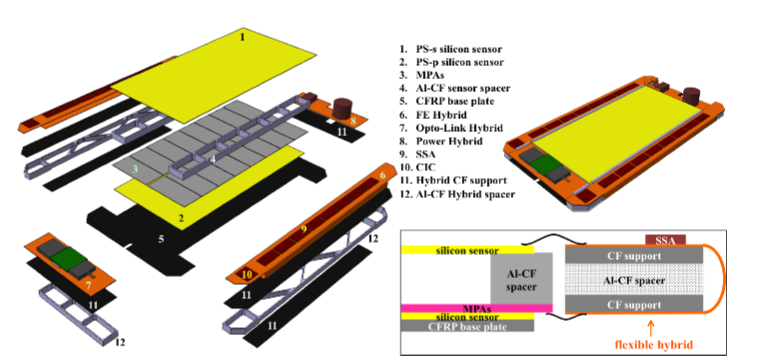
\includegraphics[width=\linewidth]{PS.png}
\caption{An exploded view of the PS module is shown.}
\label{fig:PS}
\end{figure*}




%------------------------------------------------

\section{Hardware}
The proposed automated assembly system consists of three sub-systems: the motion subsystem, the vision subsystem and the vacuum subsystem. 
The motion system provides the precise mechanical movements needed to arrange the components comprising the SSA. Movement of the components is achieved via mounting on the two moveable parts of the motion
system: the x-y-z and rotation stages. An custom-built AL tool known as the \emph{arm} is mounted on the x-y-z stage allowing mounting of components and thus movement of components in Cartesian coordinates. Components placed on the rotation stage may rotate in the horizontal plane with an angle $\phi$. The motion stages are controlled by a motion controller unit. All motion hardware is manufactured by Lang \footnote{Lang models: GT9-NSMA, LT-LBMA, RT5-NSMA} with motion precisions of 4 $\mu$m and $2$ mrad respectively. 

The vacuum system enables the mounting of components to the arm and rotation stage. It consists of a single pump providing vacuum to four switchable valves which in turn distribute vacuum to independent vacuum lines. The valves are switched to on(off) states by applying a control signal of 12 (0)V. The 12V signals are provided by a relay card. One vacuum line connects to the a \emph{pickup tool} which is mounted on the arm. The pickup tool consists of an ESD plastic block housing an inner vacuum chamber which distributed the vacuum to an array of downward facing suction cups which slightly protrude below the bottom side of the tool. A diagram of the pickup tool is shown in figure \ref{fig:pickuptool}. The \emph{pickup} procedure is performed by contacting the suction cups with the sensor, and switching 
on the vacuum within the pickup tool. The \emph{setdown} procedure is performed by contacting the mounted sensor with the lower surface on which the component will be placed, switching off the vacuum in the pickup tool and moving the arm away. In order to avoid any movement of the component as the arm moves away, the component will be fixed in its setdown position with a separate array of upward-facing suction cups and independent vacuum line.


The vision system acquires images of components allow determination of their positions and orientations which is crucial for precise assembly. The vision system consists of two high-resolution cameras \footnote{IDS models}. One camera is mounted on the arm and is referred to as the \emph{mobile camera}. The other is mounted on a fixed vertical bracket in the assembly area and is known as the \emph{stationary camera}. Both cameras are fixed in a downward-facing orientation. The mobile camera acquires images immediately before pickups and immediately after setdowns in order to determine the positions of unmounted components. Conversely, the stationary camera acquires images of the sensors after pickups and before setdowns in order to determine their mounted orientation.


\section{Software}
The control of the motion, vision and vacuum subsystems is integrated in a single software application henceforth referred to as \emph{PSAuto} \footnote{htps:github.com://}.  PSAuto is entirely written in C++ and utilises the Qt framework version 4.8.7.  A schematic illustrating the integration of the subsystems with PSAuto is shown in figure \ref{fig:PSAuto}.



\subsection{Pattern recognition}




\section{Methods}

\begin{figure}[ht]\centering % Using \begin{figure*} makes the figure take up the entire width of the page
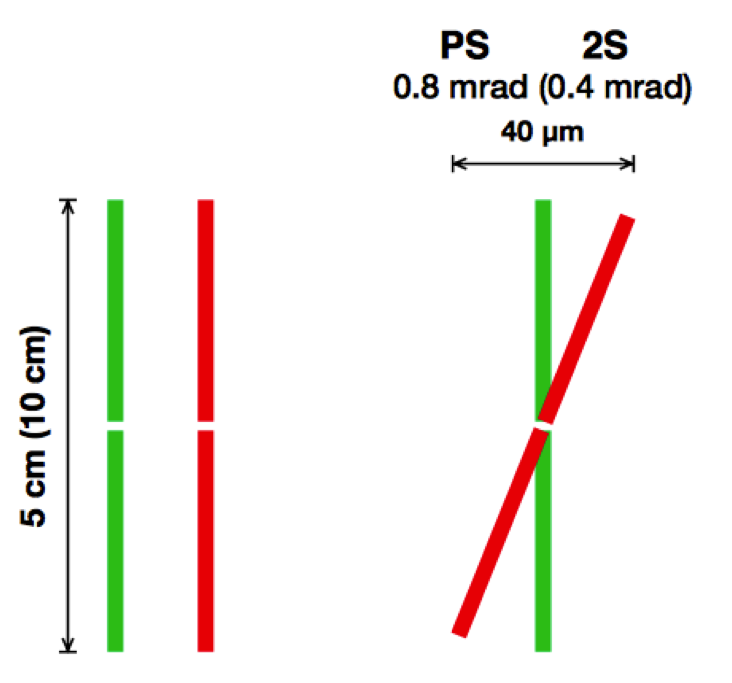
\includegraphics[width=0.5\linewidth]{Precision.png}
\caption{The precision requirements of the assembly of PS and 2S modules are shown.}
\label{fig:precision}
\end{figure}


\begin{figure}[ht]\centering % Using \begin{figure*} makes the figure take up the entire width of the page
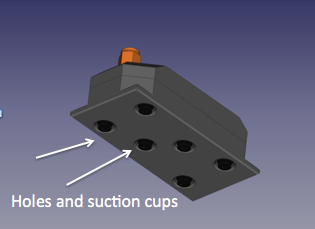
\includegraphics[width=\linewidth]{pickuptool.png}
\caption{DES}
\label{fig:pickuptool}
\end{figure}


\begin{figure}[ht]\centering % Using \begin{figure*} makes the figure take up the entire width of the page
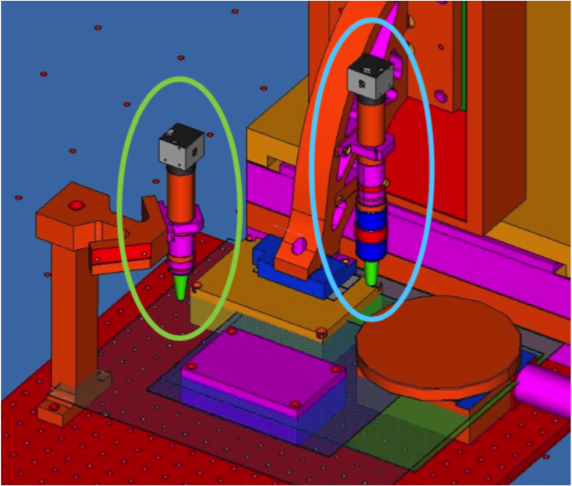
\includegraphics[width=\linewidth]{CADSetup.png}
\caption{DES}
\label{fig:cadsetup}
\end{figure}


\lipsum[4] % Dummy text

\begin{equation}
\cos^3 \theta =\frac{1}{4}\cos\theta+\frac{3}{4}\cos 3\theta
\label{eq:refname2}
\end{equation}

\lipsum[5] % Dummy text

\begin{enumerate}[noitemsep] % [noitemsep] removes whitespace between the items for a compact look
\item First item in a list
\item Second item in a list
\item Third item in a list
\end{enumerate}

\subsection{Subsection}

\lipsum[6] % Dummy text

\paragraph{Paragraph} \lipsum[7] % Dummy text
\paragraph{Paragraph} \lipsum[8] % Dummy text

\subsection{Subsection}

\lipsum[9] % Dummy text

\begin{figure}[ht]\centering
\includegraphics[width=\linewidth]{results}
\caption{In-text Picture}
\label{fig:results}
\end{figure}

Reference to Figure \ref{fig:results}.

%------------------------------------------------

\section{Open tasks}

\subsection{Design and production of the assembly platform}

\subsection{}

\subsection{Alignment Metrology}

\lipsum[10] % Dummy text

\subsection{Subsection}

\lipsum[11] % Dummy text

\begin{table}[hbt]
\caption{Table of Grades}
\centering
\begin{tabular}{llr}
\toprule
\multicolumn{2}{c}{Name} \\
\cmidrule(r){1-2}
First name & Last Name & Grade \\
\midrule
John & Doe & $7.5$ \\
Richard & Miles & $2$ \\
\bottomrule
\end{tabular}
\label{tab:label}
\end{table}

\subsubsection{Subsubsection}

\lipsum[12] % Dummy text

\begin{description}
\item[Word] Definition
\item[Concept] Explanation
\item[Idea] Text
\end{description}

\subsubsection{Subsubsection}

\lipsum[13] % Dummy text

\begin{itemize}[noitemsep] % [noitemsep] removes whitespace between the items for a compact look
\item First item in a list
\item Second item in a list
\item Third item in a list
\end{itemize}

\subsubsection{Subsubsection}

\lipsum[14] % Dummy text

\subsection{Subsection}

\lipsum[15-23] % Dummy text

%------------------------------------------------
\phantomsection
\section*{Acknowledgments} % The \section*{} command stops section numbering

\addcontentsline{toc}{section}{Acknowledgments} % Adds this section to the table of contents

So long and thanks for all the fish \cite{Figueredo:2009dg}.

%----------------------------------------------------------------------------------------
%	REFERENCE LIST
%----------------------------------------------------------------------------------------
\phantomsection
\bibliographystyle{unsrt}
\bibliography{sample}

%----------------------------------------------------------------------------------------

\end{document}